

\documentclass[reprint,english,notitlepage]{revtex4-1}  % defines the basic parameters of the document

% if you want a single-column, remove reprint

% allows special characters (including æøå)
\usepackage[utf8]{inputenc}
\usepackage[english]{babel}


\newcommand*{\QEDA}{\hfill\ensuremath{\blacksquare}}
\usepackage{amsmath, amssymb}

%% note that you may need to download some of these packages manually, it depends on your setup.
%% I recommend downloading TeXMaker, because it includes a large library of the most common packages.

\usepackage{physics,amssymb}  % mathematical symbols (physics imports amsmath)
\usepackage{graphicx}         % include graphics such as plots
\usepackage{xcolor}           % set colors
\usepackage{hyperref}    
\usepackage{filecontents}
% automagic cross-referencing (this is GODLIKE)
\usepackage{tikz}             % draw figures manually
\usepackage{listings}         % display code
\usepackage{subfigure}        % imports a lot of cool and useful figure commands



% defines the color of hyperref objects
% Blending two colors:  blue!80!black  =  80% blue and 20% black
\hypersetup{ % this is just my personal choice, feel free to change things
    colorlinks,
    linkcolor={red!50!black},
    citecolor={blue!50!black},
    urlcolor={blue!80!black}}

%% Defines the style of the programming listing
%% This is actually my personal template, go ahead and change stuff if you want
\lstset{ %
	inputpath=,
	backgroundcolor=\color{white!88!black},
	basicstyle={\ttfamily\scriptsize},
	commentstyle=\color{magenta},
	language=Python,
	morekeywords={True,False},
	tabsize=4,
	stringstyle=\color{green!55!black},
	frame=single,
	keywordstyle=\color{blue},
	showstringspaces=false,
	columns=fullflexible,
	keepspaces=true}

%% USEFUL LINKS:
%%
%%   UiO LaTeX guides:        https://www.mn.uio.no/ifi/tjenester/it/hjelp/latex/ 
%%   mathematics:             https://en.wikibooks.org/wiki/LaTeX/Mathematics

%%   PHYSICS !                https://mirror.hmc.edu/ctan/macros/latex/contrib/physics/physics.pdf

%%   the basics of Tikz:       https://en.wikibooks.org/wiki/LaTeX/PGF/TikZ
%%   all the colors!:          https://en.wikibooks.org/wiki/LaTeX/Colors
%%   how to draw tables:       https://en.wikibooks.org/wiki/LaTeX/Tables
%%   code listing styles:      https://en.wikibooks.org/wiki/LaTeX/Source_Code_Listings
%%   \includegraphics          https://en.wikibooks.org/wiki/LaTeX/Importing_Graphics
%%   learn more about figures  https://en.wikibooks.org/wiki/LaTeX/Floats,_Figures_and_Captions
%%   automagic bibliography:   https://en.wikibooks.org/wiki/LaTeX/Bibliography_Management  (this one is kinda difficult the first time)
%%   REVTeX Guide:             http://www.physics.csbsju.edu/370/papers/Journal_Style_Manuals/auguide4-1.pdf
%%
%%   (this document is of class "revtex4-1", the REVTeX Guide explains how the class works)


%% CREATING THE .pdf FILE USING LINUX IN THE TERMINAL
%% 
%% [terminal]$ pdflatex template.tex
%%
%% Run the command twice, always.
%% If you want to use \footnote, you need to run these commands (IN THIS SPECIFIC ORDER)
%% 
%% [terminal]$ pdflatex template.tex
%% [terminal]$ bibtex template
%% [terminal]$ pdflatex template.tex
%% [terminal]$ pdflatex template.tex
%%
%% Don't ask me why, I don't know.
\begin{document}
\title{FYS-STK 4155 Project 3 H22\\
Prediction of Heart Disease Diagnosis with Neural Network and Random Forest machine learning models} \\ 
\large{}
\author{Lasse Totland, Domantas Sakalys, Synne Mo Sandnes & Semya A. Tønnessen}
\date{\today}      % self-explanatory
\noaffiliation                            % ignore this
\begin{abstract} 
This report covers the development of two binary classification machine learning models for prediction of heart disease diagnosis using the 1988 Cleveland Clinic Foundation survey data on heart disease among hospital patients. The data set contains 14 attributes relevant to our analysis and we determined that none of them should be extracted during preprocessing as all of them contributed positively on the prediction test accuracy of our models. Using a classification Feed Forward Neural Network with back-propagation (and activation functions RELU for one hidden layer and softmax for output layer) we achieved an accuracy of up to $91\%$ with learning rate $\eta = 0.01$ and regularization factor $\lambda = 0.01$ using hyperparameter analysis. Using a Random Forest Classifier with Adaptive Boosting (500 estimators) we achieved a test accuracy of $88\%$ with $\eta = 0.1$ and max tree depth of $1$ using hyperparameter analysis, as well as a $89\%$ true positive prediction accuracy. These results are comparable with established literature analysing the same data set.
\end{abstract}                           

\maketitle                                % creates the title, author, date & abstract



\section{Introduction}

Data science and machine learning tools can be useful in the medical field. They support complex clinical decision-making and could be helpful in the prediction of various ailments, such as heart decease where risk factors such as high blood pressure and cholesterol can be considered. 
While there are still barriers to adopting machine learning in the medical field, such as lack of resources and the importance of finding  suitable mathematical models, in addition to privacy concerns, the method has considerable potential to transform healthcare. 
\vspace{3mm}
\\ 
Heart disease refers to a group of conditions that affect the heart. According to World Health Organization data, cardiovascular diseases are now the leading cause of mortality globally, accounting for 17.9 million deaths per year \cite{who}. Various harmful activities, such as an unhealthy diet, use of tobacco, lack of physical activity and alcohol abuse, can increase the risk of heart disease. Other factors that may rise the risk are excessive cholesterol, obesity, increased triglyceride levels, hypertension, high bloodsugar and so on \cite{who}. The American Heart Association cites some symptoms such as sleep problems, an increase and drop in heart rate (irregular heartbeat), swollen legs, and in certain cases rapid weight gain \cite{heartorg}. All of these symptoms mirror various diseases, such as those seen in the elderly, making it difficult to establish a precise diagnosis, which might lead to death in the near future. 
\vspace{3mm}
\\ 
In this study, we aim to predict the presence of heart disease in patients using machine learning techniques. We used the 1988 Heart Disease data set from the Cleveland Clinic Foundation, which consists of 297 patients and 14 features. Our approach involved training a feedforward neural network and a decision tree on this data set to classify patients as either having heart disease or not. Through our analysis, we sought to determine which of these two models would be more effective at predicting heart disease in this population.
\vspace{3mm}
\\ 
When evaluating the final models we will compare their performance with established literature studying the same data set. The research article we compare with achieved test accuracies of $88\%$ using Random Forest classification and $86.8\%$ using Deep Learning classification \cite{Bharti_et_al}.
\vspace{3mm}
\\ 
In section~\ref{sec: theory} we introduce the relevant theory in detail. The data set and preparation are presented in section~\ref{sec: method}, as well as the models that have been used. Our results and a discussion of these are presented in section~\ref{sec: results}, before we go over the conclusion and final outlook in section~\ref{sec: conclusion}. 

All python code referred to in this report can be found in the GitHub repository located at \url{https://github.com/lassetotl/fys-stk/tree/main/project\%203}.

\section{Theory}\label{sec: theory}

\subsection{Bivariate correlation}
\label{theory:corr}
In statistics, bivariate correlation is a measure of linear correlation between two sets of data. If the values of one set increases as the other one also increases, then they have significant positive linear correlation. If one \textit{decreases} as the other increases they have negative linear correlation. The formula for bivariate correlation will thus score positive or negative values in the range $r_{xy} \in [-1,\ 1]$ (values close to 0 will have no significant correlation), and is defined by the Pearson method for data sets x and y as:

\begin{equation}
\resizebox{.8\hsize}{!}{ %Scaling equation
    r_{xy} = \dfrac{\sum_{i=1}^n(x_i - \bar{x})(y_i - \bar{y})}{\sqrt{\sum_{i=1}^n (x_i - \bar{x})^2 \sum_{i=1}^n (y_i - \bar{y})^2}}},
\end{equation}

where $n$ is sample size, $x_i$ and $y_i$ are sample points of index $i$ and $\bar{x}$ and $\bar{y}$ are the sample mean values of each set \cite{pearson}. 


\subsection{Feed Forward Neural Network}
A Feed Forward Neural Network (FFNN) is a neural network that processes data in one direction. We feed it with an input, and the network processes the input to the output. This happens without any loops. The weights and biases of the connections between neurons and layers are adjusted during the training that minimizes error between the predicted and desired output. One example of a task where this type of network is used, is a classification task. The algorithm was previously discussed in further detail in project 2~\cite{proj2}.

\subsection{Hyper parameters}\label{theory:hyper-parameters}
The regularization factor $\lambda$ is used to control the complicity of the model. It adds a penalty term to the loss function when it is being optimized during the training process. One common form of regularization is called L2 regularization, which adds a penalty term to the loss function which is proportional to the sum of the square of the weights, and this is the type of regularization used in our method. 
This regularization is important in neural network training, as it can help to prevent overfitting and improve the performance of the model. This means that by adding a regularization term to the loss function, the model is "encouraged" to find balance between fitting the training data well and keeping the complexity of the model under control. 
We have written about the theory on mini-batch sizing in detail in project 2~\cite{proj2}. 


\subsection{ADAM optimizer}\label{Adam}
Adaptive Moment Estimator (ADAM) is an optimization algorithm that is used in training neural networks. In our case, this optimizer is used to train our feed forward neural network. The principle of ADAM is to combine the ideas of stochasctic gradient descent (SGD) and momentum optimization by using moving averages of the parameters to provide a running estimate of the second raw moments of the gradients. This means that the algorithm "adapts" the learning rates of each parameter based on the historical gradient information.

\subsection{Decision trees}
Decision trees are supervised learning algorithms used in classification and regression tasks. The method is typically divided into a root node, the interior nodes, and the final leaf nodes, which are all connected by what we refer to as branches. 
The goal is to create a model which can predict the value of a target variable by learning simple decision rules which are inferred from the data features. The most informative descriptive features are those which reproduce the best output features. The process of finding this feature is continued until we find a stopping criteria where we end up in the leaf nodes. 
\vspace{3mm}
\\ 
There are several advantages to using decision trees. The visualization of a tree makes the method easy to understand and interpret. In addition, tree models can handle both continuous and categorical data, can model nonlinear relationships, and can model interactions between the different descriptive features~\cite{morten}. 
Unfortunately, trees often have a lower level of predictive accuracy than some other approaches. The method is also prone to overfit data. However, by aggregating decision trees with methods such as bagging, random forests, and boosting, the predictive performance of trees can be improved. 

\subsection{The CART algorithm}
\label{CART_algo}
There are several different algorithms that generate trees differently. In this report we will discuss the CART algorithm used in the {\lstinline[language={[python]TeX}, basicstyle=\ttfamily]|scikit-learn|} decision tree python modules \cite{morten}. 
\vspace{3mm}
\\ 
The Classification and Regression Tree (CART) algorithm grows decision trees with structures like we can see in Figure \ref{fig:CART}, where the root and internal nodes split to a maximum of two new nodes. Proceeding downwards leads to a leaf node and a prediction of class 1 or 2.
\begin{figure}[h!]
    \centering
    \includegraphics[scale = 0.36]{CARTClassificationAndRegressionTree.jpg}
    \caption{Hypothetical CART binary classification decision tree structure with color coded outcomes in the leaf nodes \cite{CART}.}
    \label{fig:CART}
\end{figure}
\vspace{3mm}
\\ 
The core of the algorithm is deciding how the branches should be split depending on the attributes of the input data. For a single tree, the algorithm will choose some attributes and attempt to divide the distribution of classes in the data into different regions. To get 'pure nodes', these regions should ideally exclusively contain data relating to either class 1 or 2 but a more realistic case is that it manages to define regions with a clear majority.
\vspace{3mm}
\\ 
Thus, when the tree classifies a specific data set, each node in the tree basically evaluates which region in the same distribution space (focusing on the same attributes) the instance should fall under, and then conclude the classification following the majority vote in the region.
\vspace{3mm}
\\ 
The algorithm also seeks to minimize error in the leaf nodes by minimizing variance in the defined region, and may define a new region (and thus a new split in the tree) if a certain criteria is met. For this project the 'entropy' criterion $s \in [0, \ 1]$ is relevant, which evaluates the disorder within a specific region and is defined as:
\begin{equation}
    s = - \sum_{k=1}^K p_{mk} \log p_{mk},
\end{equation}
where $K$ is the amount of classes and $p_{mk}$ is the amount of outcomes of the class $k$ in a given region. 
\vspace{3mm}
\\ 
For a binary case we use $K = 2$ and the range becomes $s \in [0, \ 1]$ where the minimum means we can split into a pure node and the maximum means that the probability of class 1 and class 2 is the exact same (maximum disorder). The growing of the tree will persist until the entropy is sufficiently low. 

\subsection{Random forest algorithm}
Plain decision trees suffer from high variance, where the data is prone to overfitting. Bootstrap aggregation (bagging), is a procedure for reducing the variance of a statistical learning method, and typically results in improved accuracy over prediction using a single tree. However, it can be challenging to interpret the resulting model. Random forests improve bagging by implementing a small tweak that decorrelates the trees. 
\vspace{3mm}
\\ 
We build a number of decision trees on bootstrapped training samples. Each time a split in a tree is considered, a random sample of $m$ predictors is chosen as split candidates from the full set of $p$ predictors. This split only uses one of the $m$ predictors and the algorithm will not consider a majority of the available predictors~\cite{morten}. At each split, a fresh sample of $m$ predictors is taken, typically 
\begin{align}
    m \approx \sqrt{p}. 
\end{align}
This prevents the bagged trees from all being similar to one another by not favoring one strong predictor which is always used in the top split, overshadowing the other moderately strong predictors. 
\vspace{3mm}
\\ 
% Algorithm 
In order to build the algorithm, we assume that we grow a forest of $B$ trees. For $b=1:B$ we then draw a bootstrap sample from the training data organized in the $\mathbf{X}$ matrix and grow a random forest tree $T_b$ based on the bootstrapped data by repeating three steps: 
\begin{enumerate}
    \item Select $m\leq p$ variables at random from the $p$ predictors 
    \item Pick the optimal split among the $m$ features using an algorithm (for example the CART algorithm), and create a new node. 
    \item Split the node into daughter nodes. 
\end{enumerate}
\vspace{3mm}
\\ 
The steps are repeated until the maximum node size is obtained. Finally, we can output the ensemble of trees ${T_b}^B_1$ and make predictions for the problem. 


\subsection{Boosting method}
The boosting method combines weak classifiers by applying the weak classifier to modify the data, in order to modify the data and create a better classifier. This is done for several iterations, for which we emphasize the observations which are misclassified by weighting them with a factor. 
\vspace{3mm}
\\ 
The principle is very similar to standard random forests except that after iterating, the trees that showed the fewest misclassifications will weigh more significantly on the classification voting. The process of updating these tree-specific weights over a number of iterations corresponds to a Gradient Descent algorithm which is a topic we have discussed in detail in report 2~\cite{proj2}.

\section{Method}\label{sec: method}

\subsection{Data Set Description}

For our analysis we are using the 1988 Heart disease data set from the Cleveland Clinic Foundation containing data on 297 patients including their diagnosis (1 = disease, 0 = no disease). The set includes 137 positive diagnoses, 160 negative \cite{heart}.
\vspace{3mm}
\\ 
The initial study contained 76 measured attributes, but all published experiments referring to the data only make use of 14 attributes, including the diagnosis. The remaining are documented as:

\begin{enumerate}
    \item sex - (1 = male, 0 = female)
    \item age - patient age in years
    \item cp - chest pain type (1-4)
    \item trestbps - resting blood pressure (in mm Hg on admission to hospital)
    \item fbs - fasting blood sugar $<$ 120 mg/dl (1 = true, 0 = false)
    \item chol - cholesterol measure in mg/dl 
    \item restecg - ecg observation at resting condition (0-2)
    \item thalach - maximum heart rate achieved
    \item exang - exercise induced angina (1 = True, 0 = False)
    \item oldpeak - ST depression induced by exercise relative to rest
    \item slope - slope of the peak exercise ST segment
    \item ca - number of major vessels (0-3) colored by flouroscopy
    \item thal - 3 = normal, 6 = fixed defect, 7 = reversable defect
\end{enumerate}
\vspace{3mm}
\\ 
In our analysis we use this selection. The UCI archive contains further attribute documentation~\cite{heart}. Some features (like blood pressure levels) are numerical, and some are categorical. However, we are going to use a modified version of the Cleveland data set ('$heart\_cleveland\_upload.csv$'~\cite{heart_csv}) that has already relocated each feature category to their numerical values (0 and 1 instead of False and True and so on).
\vspace{3mm}
\\
The scatter plots for some of the numerical features in figure \ref{fig:scatter1} gives an impression of the data variety and distribution between positive and negative diagnoses. 
\begin{figure}[h!]
    \centering
    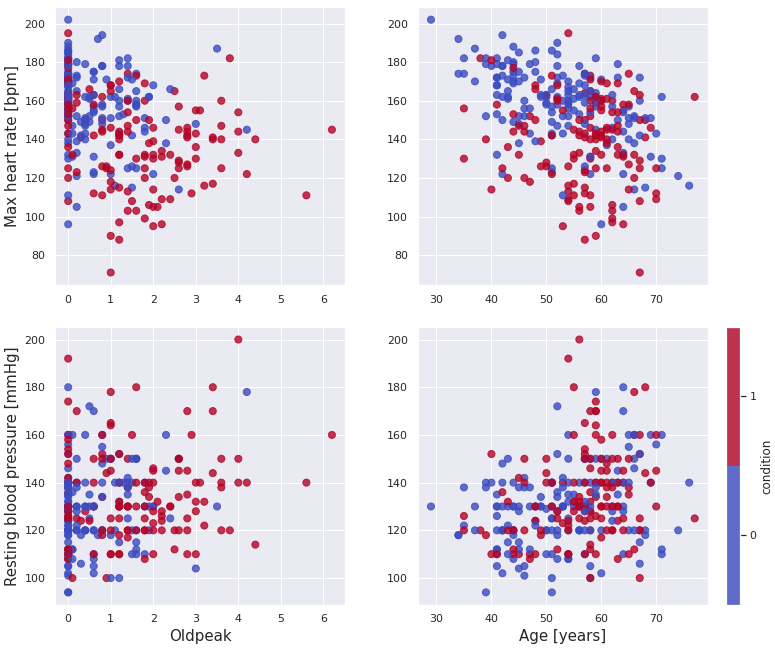
\includegraphics[scale = 0.335]{Heart_Scatter.png}
    \caption{Scatter plots of the attributes Age, Oldpeak, Trestbps (Resting blood pressure) and Thalach (Max heart rate), with condition (1 = positive or 0 = negative diagnosis) color-coded for the corresponding patient.}
    \label{fig:scatter1}
\end{figure}

\subsection{Data preparation}

Before proceeding with the analysis we need to have a proper look at our data, and potentially smooth out any errors if needed. 
\vspace{3mm}
\\
We will calculate a correlation matrix using the Pearson method, as defined in theory section~\ref{theory:corr} and implemented with the pandas python module {\lstinline[language={[python]TeX}, basicstyle=\ttfamily]|dataframe.corr|}, and consider extracting features with little correlation to the diagnosis from the data set. 
Other correlations will also be discussed briefly to get further insight into the data set, as well as verify that the correlations seem qualitatively correct taking into account external literature on cardiology as a way to prove that the data has been imported and handled correctly.
\vspace{3mm}
\\
The prepared data set will be split into a training set ($80\%$) that is used to train our models and a test set (20\%) which will be a target for the models to evaluate their accuracy with.
\vspace{3mm}
\\
In this data set we have a matrix that represent features and its values, and a target array which tells us if the patient has a heart disease or not. For the neural network analysis we use one-hot encoding to convert these target values from single integers into binary representation. This means that statement 1 would become (0,1), and 0 would be (1,0).
This one-hot encoding ensures that machine learning does not assume that higher numbers are more important.

\subsection{Neural network analysis}
Feed Forward Neural Network (FFNN) will be the first machine learning method that we will apply to the data-set. We will start off by writing our own FFNN algorithm, and then compare the results by using TensorFlow python module.
\vspace{3mm}
\\
When defining the neural network architecture, we define a network that consist of an input layer, one or more hidden layers, and an output layer. The input layer contains a number of neurons equal to the number of the features. In our case, we have 13 features. The hidden layer containes a number of neurons determined based on the complexity of the data. However, we will be using 90 neurons and one hidden layer as a starting point. We will then try different values and see how our neural network performs. Since this is a classification problem, meaning that we either have a true or false statement for a patient having a heart disease, our output layer contains a single neuron. This neuron will have value of 0 indicating the absence of heart disease and a value of 1 indicating the presence of heart disease.
\vspace{3mm}
\\
When writing our own script for FFNN, we also have to  define some hyper-parameters. These hyper-parameters are
\begin{itemize}
    \item Regularization parameter $\lambda$
    \item The size of mini-batch
    \item Learning rate.
\end{itemize}
See theory section \ref{theory:hyper-parameters} for a description of each of these hyper-parameters. As a starting point, we will be using batches with size of 50 random data-points. As for the regularization parameter $\lambda$ and learning rate, we will perform a grid search. 
To do this, we define two lists containing values from -5 to 7 with a step of 1 on a logarithmic scale. We then make two for loops that runs over all the values from these lists and performs our FFNN and calculates the accuracy score for each of these values. This way, we can map out the values of learning rate and $\lambda$ that fit the best with our data.
\vspace{3mm}
\\
The activation function of the neurons in the hidden layer is determined based on the type of data and desired behavior of the network. Since this is a binary classification task, we are using the Sigmoid \cite{proj2} activation function. These activation's are then used in the output layer, where we perform Softmax function \cite{proj2} to determine the probability for the patient to have a heart disease. Since this is a classification problem, we use this probability and return a statement 1 if the probability is higher than 0.5, and 0 if it is lower than 0.5.
\vspace{3mm}
\\
However, in order to train FFNN, we need an optimizer to find the best values for weights for each neuron and bias for the hidden layer. In order to do this, we use Stochastic gradient descent with momentum (See \cite{proj2} theory section B) in backpropagation. This means that we calcculate the error of output, and accordingly to the error, we backpropagate and change the values of weights and biases.
\vspace{3mm}
\\
We wish to compare the results with TensorFlow built in library. Therefore, we first import the library, and define input and target data and feed it to the library. Once again we use one-hot decoding for the targets. 
\vspace{3mm}
\\
We also wish to experiment with different architectures by trying out different number of hidden layers, and different number of neurons for each layers. Additionaly, we wish to test out different activation functions such as Sigmoid, ReLu, Tanh and softmax function. We will be also testing different optimizers, such as Stochastic gradient descent (SGD), Adam, RMSprop and Adagrad. 




\subsection{Random forest analysis}
For the second model we will develop a random forest classifier using adaptive boosting with scikit-learn python modules, and using our prepared data set with no exctracted features. The models will use the 'entropy' criterion when splitting trees as established section~\ref{CART_algo}.
\vspace{3mm}
\\
The optimal learning rate $\eta$ and max depth of the aggregated decision trees will be determined with hyperparameter analysis by calculating the accuracy from models of various configurations and presenting these accuracies in a heatmap.
\vspace{3mm}
\\
The highest scoring configuration will be used to generate a confusion matrix to evaluate the final model's true and false positive/negative test prediction accuracy after being trained by the training data that we have prepared. The confusion matrix simply compares how many positive and negative diagnoses that our model gives correctly, and normalizes to give accuracy values between 0 and 1. 
\vspace{3mm}
\\
The total accuracy score will be calculated, and we will use the same model with the data set where we extracted the 'fbs' attribute (the one with 0.00 correlation with the patient condition) to see if there is a significant change in accuracy.

\section{Results \& Discussion}\label{sec: results}

\subsection{Results of initial data set analysis}

Figure \ref{fig:corr} shows the correlation matrix for the features in the heart disease data set. The diagonal elements were removed because they would score a perfect 1 and de-saturate the color scale for the other positive correlations. The upper triangle was removed because it is symmetric with the lower and therefore redundant.
\begin{figure}[h!]
    \centering
    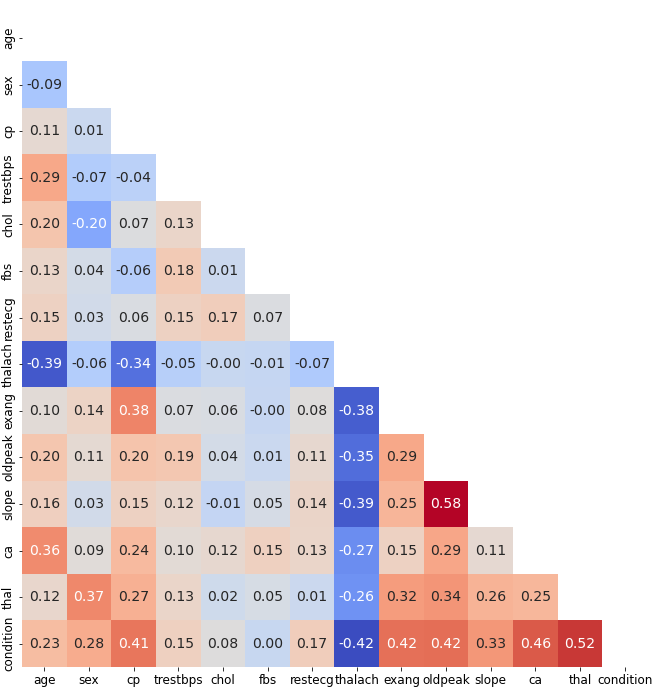
\includegraphics[scale = 0.37]{Corr_Heatmap.png}
    \caption{Correlation matrix for the relevant features in the UCI heart disease data set. The blue elements display negative correlation and the red positive correlation.}
    \label{fig:corr}
\end{figure}
\vspace{3mm}
\\
Some correlations of note are that age has a positive correlation with chol $(0.20)$ and condition $(0.23)$, implying that the older patients in the survey had higher cholesterol levels and were more likely to be diagnosed with heart disease. Age also has a significant negative correlation with thalach $(-0.39)$, implying that maximum heart rate decreases with patient age. These observations agree qualitatively with literature on cardiology and aging \cite{heart_age} so we assume that we have imported and handled the data set correctly.
\vspace{3mm}
\\
When constructing our machine learning models we are most interested in the bottom row of the heatmap which shows us the correlation between the various features and the condition, and we do see a fair amount of significant positive/negative correlations over $0.4$, meaning they are important for predicting the diagnosis.
\vspace{3mm}
\\
The attribute for fasting blood sugar 'fbs' scores 0.00 correlation even though it has a stronger correlation to other features. The data set isn't huge so deciding whether or not to extract this feature should not affect the model performance a lot, but we will make separate processed data sets that include all features and one that excludes fbs to see if it affects the prediction accuracy.

\subsection{FFNN results}
By writing our own Feed Forward Neural network, and doing a grid search for the most optimal learning rate and regularization factor $\lambda$ value, we find that the most optimal learning rate has value of 0.00001, and $\lambda$ has value 0.01, which gives an accuracy of 56\%. Table \ref{table:grid-search} shows the accuracy rate for other values that we have picked.
\\
\begin{table}[h!] %%h! er for å tvinge tabellen til å være nærmest mulig her i dokumentet
  \begin{center}
    \caption{Grid search for optimal $\lambda$ and learning rate with the corresponding accuracy rate for FFNN analysis} %Tabelltekst
    \label{table:grid-search}
    \begin{tabular}{l|c|r } % for hver kolonne har du {a|b|c} der a er for 1.kolonne, b for 2. kolonne etc, l=venstrestil, r=høyrestilt, c = senterstilt. Se posisjonen til tallene i de forskjellige kolonnene. Har du 4 kolonner der alle er senterstilt blir det f.eks. {c|c|c|c}
    \hline
      \textbf{Learning rate} & $\lambda$ & \textbf{Acc. rate}\\ %innhold i hver kolonne, legg til flere her hvis du har flere kolonner
      \hline %en horisontall linje for å skille overskriften fra tallene under. Vil du ha en slik linje mellom hver rad i tabellen så legg til en \hline mellom hver rad nedover her. Merk \\ er som vanlig linjeskift mens & skiller kolonner
      0.00001 & 0.01 & 0.56\\
      0.0001 & 0.01 & 0.53\\
      0.01 & 0.01 & 0.53\\
      1 & 1 & 0.53\\
      0.00001 & 0.001 & 0.38\\ 
      
    \end{tabular}
  \end{center}
\end{table}
\\
By having 56\% as accuracy rate from our FFNN, we can say that our neural network performs poorly. We have included only some of the values in table \ref{table:grid-search}, and we can see that most of them have accuracy rate of 53\%. It seems that our model guesses the output, and gets it wrong and right half of the time. This is not a good model. Additionally, since we are using stochastic gradient descent with momentum as our optimizer, we expect the learning to be a larger number than 0.00001. This is not the case here. 
\vspace{3mm}
\\
By running the gird-search multiple times, we see that the accuracy rates for the same values of hyper-parameters differ. This might be because our model is poor and it simple guesses the output randomly everytime. Meaning that in the training part where we use backpropagation to find the optimal weight and biases, we find different values for weight and biases every time. 
\vspace{3mm}
\\
We wish now to compare the results by using Tensorflow library. We have used the same architecture, and we choose to find the learning rate and the regularization factor which gave us the best results in table \ref{table:grid-search}. 
\vspace{3mm}
\\
By using tensorflow, we get \textbf{the accuracy rate up to 81\%}. However, by increasing the number of epochs, we were able to achieve higher accuracy rates. For example, when we ran the FFNN with tensorflow using 2000 epochs, we achieved an \textbf{accuracy rate of 85\%}. However, this result was not consistent across all runs. In some cases, the accuracy rate dropped back to 81\%, even with 2000 epochs. This inconsistency may be due to the random mini-batch selection used in the optimization of weights and biases. However, we observed that in most cases, we achieved accuracy to be around 85\% with higher number of epochs. 
\vspace{3mm}
\\
We wanted to optimize the architecture of our tensorflow (FFNN) by creating three lists of varying numbers of hidden layers, the number of neurons in each layer, and different sizes of mini-batches. We ran these values and found the optimal architecture. The results can be found in the file 'analyse.txt' in our github repository.
\vspace{3mm}
\\
However, we found that the high number of hidden layers and neurons does not improve FFNN. From one run, we saw that by having \textbf{1 hidden layer}, \textbf{10 neurons} on the hidden layer, and \textbf{batch size of 70} gave us the highest accuracy rate of up to \textbf{91\%}. This is higher than the $86.8\%$ achieved with deep learning in the article we referenced in the introduction.
\vspace{3mm}
\\
Additionally, we have tested different activation functions and optimizers here. We concluded that the most effective optimizer is Adam-optimizer. See theory section \ref{Adam}. As for the hidden layer activation function, we found that RELU-function is most effective. And for the output, softmax function.
\vspace{3mm}
\\
However, please note that the accuracy rate by using the same architecture and the same hyper-parameters is not the same every time we run the network. Most often we achieve an accuracy rate of 88\% up to 90\%. 


\subsection{Boosted random forest classification results}

The result from the hyperparameter analysis using the scikit-learn random forest classifier with adaptive boosting and 500 estimators, with varying learning rates $\eta$ and max depths is presented in a heatmap in Figure \ref{fig:hypertree}.
\begin{figure}[h!]
    \centering
    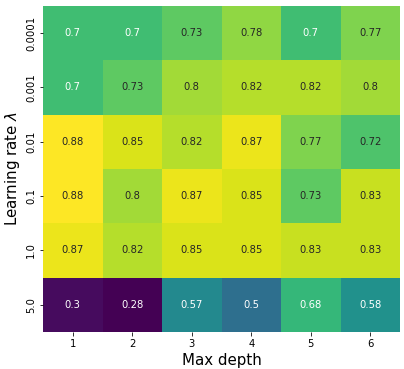
\includegraphics[scale = 0.6]{treeparameter.png}
    \caption{Prediction test accuracies from adaptive boosted random forest classification models using various hyperparameter configurations presented in a heatmap.}
    \label{fig:hypertree}
\end{figure}
\vspace{3mm}
\\
We observe from the grid search that the best performing models appear to have a max depth of 1, and learning rates $0.1$ and $0.01$ and test accuracies of $0.88$. This is the same result that was achieved with Random Forest classification in the article noted in the introduction \cite{Bharti_et_al}. When we run the model with the fbs attribute extracted, the accuracy decreases to $0.77$. 
\vspace{3mm}
\\
This implies that \textit{all} significant correlations are important in prediction models even though the attribute doesn't directly correlate with the condition. The fbs attribute (0.00 correlation with condition) has positive correlation with the attribute 'ca' which has a strong correlation with condition, and their connected relation appears to be important when constructing a prediction model of this data set as the accuracy drops when fbs is removed.
\vspace{3mm}
\\
Going back to our model trained with all the features, we generate a confusion matrix as seen in Figure \ref{fig:confusiontree}. We observe that our model has a true positive accuracy of $0.89$ and a true negative accuracy of $0.88$. This means that a given positive prediction from our model has an $89\%$ chance of being correct, and a negative prediction $88\%$.
\begin{figure}[h!]
    \centering
    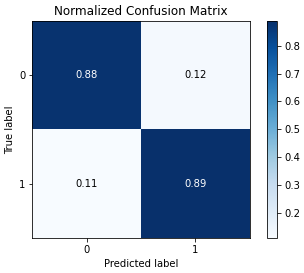
\includegraphics[scale = 0.7]{treeconfusion.png}
    \caption{Confusion matrix presenting distribution of true positive/negative and false positive/negative predictions of our final Random Forest classifier model.}
    \label{fig:confusiontree}
\end{figure}
\vspace{3mm}
\\
When performing any practical medical diagnosis, several tests may need to be performed to be confident in the result. However, it is more important that the confidence in a positive test is higher than vice versa. Take for example a covid test; a positive test has a big consequence on a person's daily routine so you want the test method to have a high true positive accuracy to avoid unnecessary diagnoses. 
\vspace{3mm}
\\
This is why the CDC (Centers for Disease Control and Prevention) in the US suggests use of covid antibody tests with specificity (true positive rate) of $\geq 99.5\%$ because of the large societal consequences of false positive diagnoses \cite{cov}.
\vspace{3mm}
\\
The difference between the true positive/negative accuracy in our case is not large, but the clinical perspective is interesting either way.

\section{Conclusion}\label{sec: conclusion}

Two machine learning models were developed in the study: a classification feedforward neural network with back-propagation, and a random forest classifier with adaptive boosting. The neural network model achieved an accuracy up to 91\% on the test set, while the random forest model achieved an accuracy of 88\% on the test set. The random forest model also had a true positive prediction accuracy of 89\%.
\vspace{3mm}
\\
However, we were not sure what exactly all attributions in the feature list do, as for example oldpeak and slope, we still managed to make them useful for the model. The model seemed to become better by including them. Meaning that we do not need a deep understanding of all the features to make a good model.
\vspace{3mm}
\\
Another point of potential improvement is that we could work with the original, untreated data. The set used in our analysis seems to have been properly pre-processed already and little work was done on it ourselves. Looking at the entire data set we could evaluate for ourselves which attributes are interesting or not, 'smoking' (True/False) is an example of a missing attribute that could prove useful. More insight into cardiology could help us determine relevant attributes more efficiently.
\vspace{3mm}
\\
We have demonstrated that the true positive accuracy in our random forest model is higher than the true negative accuracy, which is more favourable in medical diagnosis than the opposite case.
\vspace{3mm}
\\
Overall, the results of the study suggest that both the neural network and random forest models were able to achieve high levels of accuracy in predicting heart disease diagnosis using the 1988 Cleveland Clinic Foundation survey data. These results are similar to those reported in other studies that have analyzed this data set.


\bibliography{refs}
\end{document}